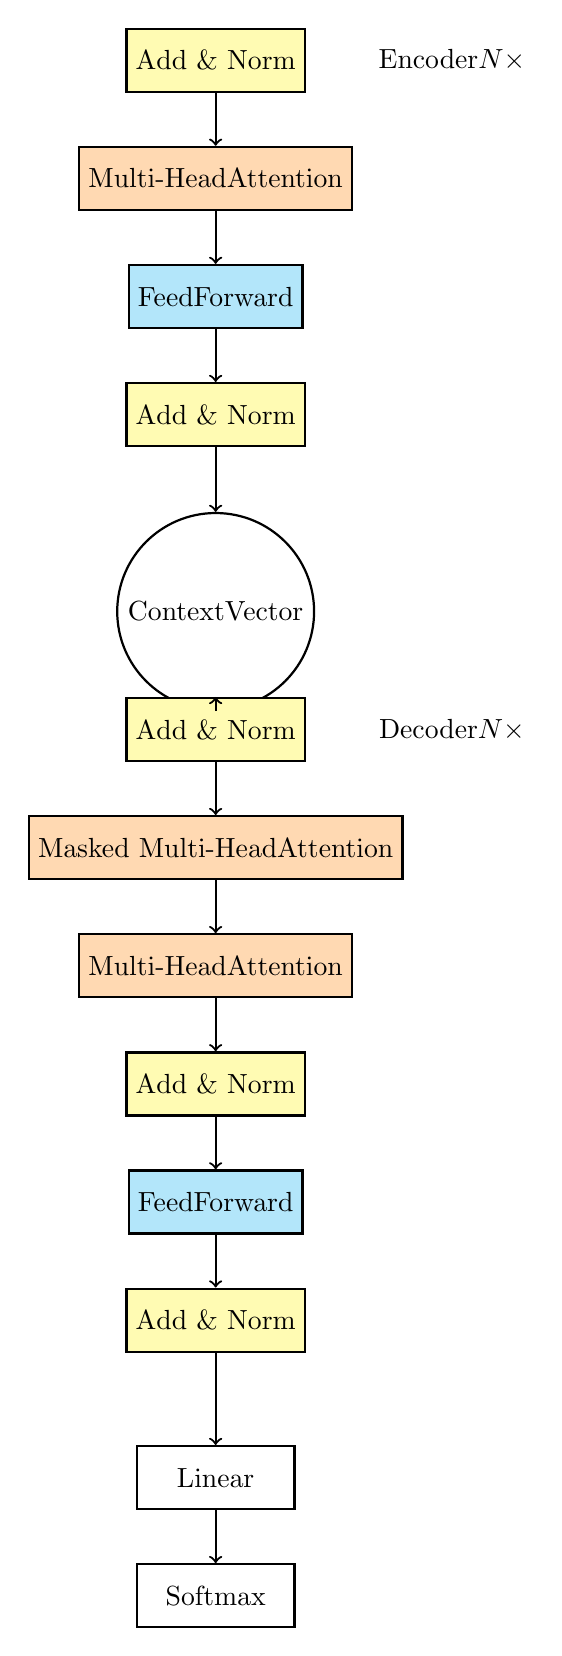
\begin{tikzpicture}[node distance=1.5cm, auto, thick]
  % Encoder block
  \node[draw, rectangle, minimum width=2cm, minimum height=0.8cm, fill=orange!30] (enc_attn) {Multi-Head\\Attention};
  \node[draw, rectangle, minimum width=2cm, minimum height=0.8cm, fill=yellow!30, above of=enc_attn] (enc_norm1) {Add \& Norm};
  \node[draw, rectangle, minimum width=2cm, minimum height=0.8cm, fill=cyan!30, below of=enc_attn] (enc_ff) {Feed\\Forward};
  \node[draw, rectangle, minimum width=2cm, minimum height=0.8cm, fill=yellow!30, below of=enc_ff] (enc_norm2) {Add \& Norm};
  
  % Encoder label
  \node[right of=enc_norm1, xshift=1.5cm] {Encoder\\$N\times$};
  
  % Context vector
  \node[draw, circle, minimum size=1cm, below of=enc_norm2, yshift=-1cm] (context) {Context\\Vector};
  
  % Decoder block
  \node[draw, rectangle, minimum width=2cm, minimum height=0.8cm, fill=orange!30, below of=context, yshift=-1.5cm] (dec_masked) {Masked Multi-Head\\Attention};
  \node[draw, rectangle, minimum width=2cm, minimum height=0.8cm, fill=yellow!30, above of=dec_masked] (dec_norm1) {Add \& Norm};
  \node[draw, rectangle, minimum width=2cm, minimum height=0.8cm, fill=orange!30, below of=dec_masked] (dec_attn) {Multi-Head\\Attention};
  \node[draw, rectangle, minimum width=2cm, minimum height=0.8cm, fill=yellow!30, below of=dec_attn] (dec_norm2) {Add \& Norm};
  \node[draw, rectangle, minimum width=2cm, minimum height=0.8cm, fill=cyan!30, below of=dec_norm2] (dec_ff) {Feed\\Forward};
  \node[draw, rectangle, minimum width=2cm, minimum height=0.8cm, fill=yellow!30, below of=dec_ff] (dec_norm3) {Add \& Norm};
  
  % Decoder label
  \node[right of=dec_norm1, xshift=1.5cm] {Decoder\\$N\times$};
  
  % Output layers
  \node[draw, rectangle, minimum width=2cm, minimum height=0.8cm, below of=dec_norm3, yshift=-0.5cm] (linear) {Linear};
  \node[draw, rectangle, minimum width=2cm, minimum height=0.8cm, below of=linear] (softmax) {Softmax};
  
  % Arrows
  \draw[->] (enc_norm1) -- (enc_attn);
  \draw[->] (enc_attn) -- (enc_ff);
  \draw[->] (enc_ff) -- (enc_norm2);
  \draw[->] (enc_norm2) -- (context);
  \draw[->] (context) -- (dec_norm1);
  \draw[->] (dec_norm1) -- (dec_masked);
  \draw[->] (dec_masked) -- (dec_attn);
  \draw[->] (dec_attn) -- (dec_norm2);
  \draw[->] (dec_norm2) -- (dec_ff);
  \draw[->] (dec_ff) -- (dec_norm3);
  \draw[->] (dec_norm3) -- (linear);
  \draw[->] (linear) -- (softmax);
\end{tikzpicture}